\documentclass[tikz, border=5pt]{standalone}
\usepackage{xstring}
\usetikzlibrary{decorations.pathreplacing,
positioning}

\newcommand{\GetBit}[2]{%
    \edef\BitPos{#2}%
    \StrLen{#1}[\StringLen]%
    \ifnum\BitPos>\StringLen
        \edef\Bit{0}%
    \else
        \StrChar{#1}{#2}[\Bit]%
    \fi
}
\newcommand{\SetBits}[1]{%
    \foreach \i in {1,...,16} {%
            \GetBit{#1}{\i}%
            \node at (\i - 0.5, 0.5) {\LARGE \textbf{\Bit}};
        }%
}

\begin{document}

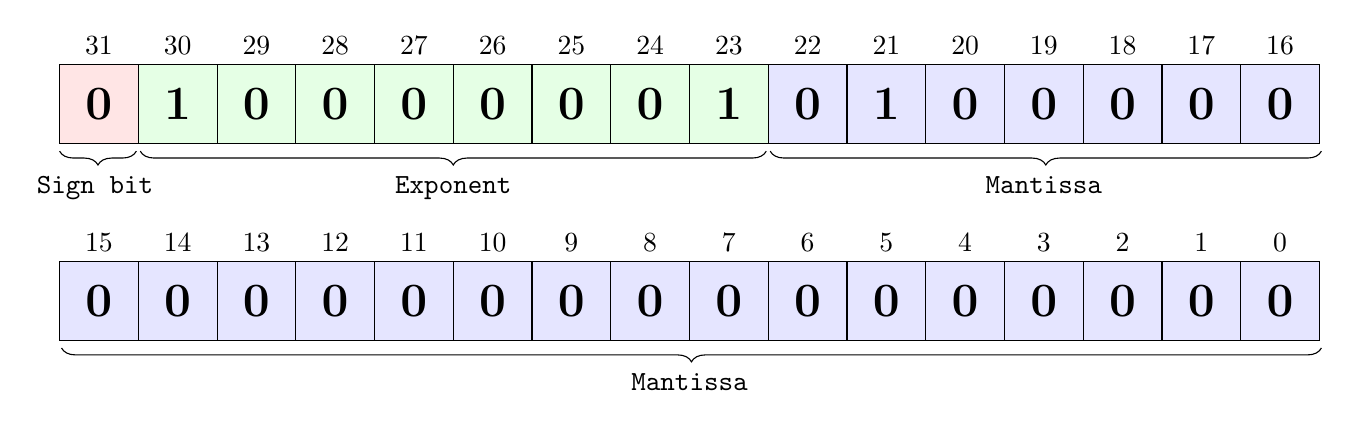
\begin{tikzpicture}

    % Colors
    \fill [red!10] (0, 0) rectangle (1, 1);
    \fill [green!10] (1, 0) rectangle (9, 1);
    \fill [blue!10] (9, 0) rectangle (16, 1);

    \foreach \i in {0,...,15} {
            % Boxes
            \draw (\i, 0) rectangle (\i + 1, 1);
        }
    \foreach \i in {16,...,31} {
            % Position
            \node [above] at (31.5 - \i, 1) {\i};
        }
    \SetBits{0100000010100000}

    % Colors
    \fill [blue!10] (0, -1.5) rectangle (16, -2.5);

    \foreach \i in {0,...,15} {
            % Boxes
            \draw (\i, -2.5) rectangle (\i + 1, -1.5);

            % Position
            \node [above] at (15.5 - \i, -1.5) {\i};
        }
    \foreach \i in {1,...,16} {%
            \GetBit{0000000000000000}{\i}%
            \node at (\i - 0.5, -2) {\LARGE \textbf{\Bit}};
        }%

    %% IEEE 754 standard
    % Signed bit label
    \draw [decorate, decoration={brace, amplitude=5pt}] (1-0.025, -0.1) -- (0, -0.1);
    \node [below] at (0.45, -0.3) {\texttt{Sign bit}};

    % Exponent label
    \draw [decorate, decoration={brace, amplitude=5pt}] (9-0.025, -0.1) -- (1+0.025, -0.1);
    \node [below] at (5, -0.3) {\texttt{Exponent}};

    % Mantissa label
    \draw [decorate, decoration={brace, amplitude=5pt}] (16+0.025, -0.1) -- (9+0.025, -0.1);
    \node [below] at (12.5, -0.3) {\texttt{Mantissa}};
    \draw [decorate, decoration={brace, amplitude=5pt}] (16+0.025, -2.5-0.1) -- (0+0.025, -2.5-0.1);
    \node [below] at (8, -2.5-0.3) {\texttt{Mantissa}};

\end{tikzpicture}

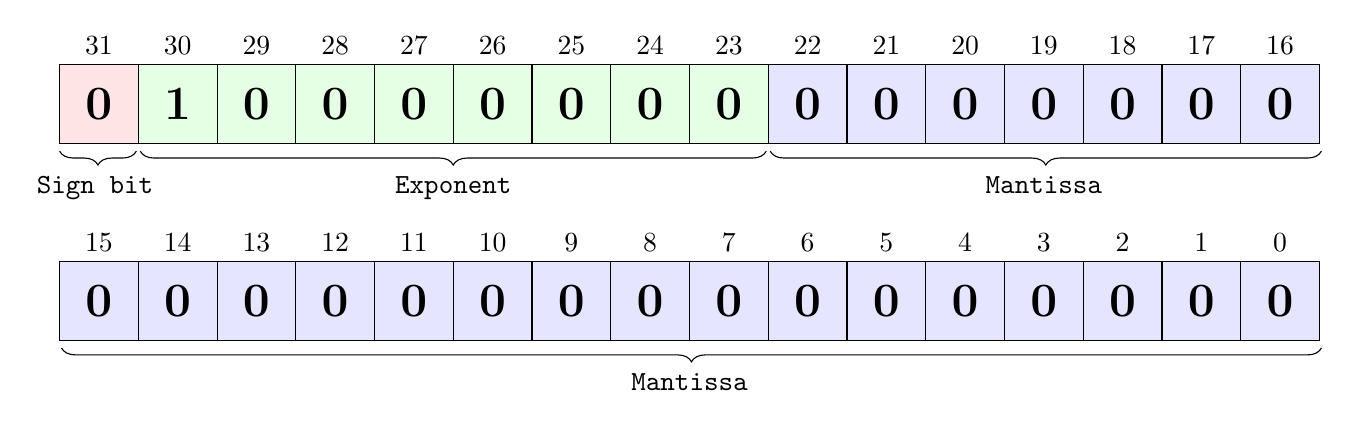
\begin{tikzpicture}

    % Colors
    \fill [red!10] (0, 0) rectangle (1, 1);
    \fill [green!10] (1, 0) rectangle (9, 1);
    \fill [blue!10] (9, 0) rectangle (16, 1);

    \foreach \i in {0,...,15} {
            % Boxes
            \draw (\i, 0) rectangle (\i + 1, 1);
        }
    \foreach \i in {16,...,31} {
            % Position
            \node [above] at (31.5 - \i, 1) {\i};
        }
    \SetBits{0100000000000000}

    % Colors
    \fill [blue!10] (0, -1.5) rectangle (16, -2.5);

    \foreach \i in {0,...,15} {
            % Boxes
            \draw (\i, -2.5) rectangle (\i + 1, -1.5);

            % Position
            \node [above] at (15.5 - \i, -1.5) {\i};
        }
    \foreach \i in {1,...,16} {%
            \GetBit{0000000000000000}{\i}%
            \node at (\i - 0.5, -2) {\LARGE \textbf{\Bit}};
        }%

    %% IEEE 754 standard
    % Signed bit label
    \draw [decorate, decoration={brace, amplitude=5pt}] (1-0.025, -0.1) -- (0, -0.1);
    \node [below] at (0.45, -0.3) {\texttt{Sign bit}};

    % Exponent label
    \draw [decorate, decoration={brace, amplitude=5pt}] (9-0.025, -0.1) -- (1+0.025, -0.1);
    \node [below] at (5, -0.3) {\texttt{Exponent}};

    % Mantissa label
    \draw [decorate, decoration={brace, amplitude=5pt}] (16+0.025, -0.1) -- (9+0.025, -0.1);
    \node [below] at (12.5, -0.3) {\texttt{Mantissa}};
    \draw [decorate, decoration={brace, amplitude=5pt}] (16+0.025, -2.5-0.1) -- (0+0.025, -2.5-0.1);
    \node [below] at (8, -2.5-0.3) {\texttt{Mantissa}};

\end{tikzpicture}

\end{document}
